\documentclass[12pt,twoside,a4paper]{article}
\renewcommand*\familydefault{\sfdefault}
\usepackage[utf8]{inputenc}
\usepackage[T1]{fontenc}
\usepackage[ngerman]{babel}
\usepackage[left=3cm,right=3cm,top=2cm,bottom=4cm]{geometry}
\usepackage{graphicx}
\usepackage{helvet}
\renewcommand{\familydefault}{\sfdefault}
\linespread{1.25}
\usepackage{xcolor}
\usepackage{hyperref}
\hypersetup{
    colorlinks,
    linkcolor={black!},
    citecolor={blue!50!black},
    urlcolor={blue!50!black}
}
\definecolor{light-yellow}{RGB}{255, 255, 204}
\usepackage[numbib,nottoc]{tocbibind}
\usepackage{caption}
\usepackage{verbatimbox}
\usepackage{apacite}
\usepackage[acronym]{glossaries}
\makeglossaries
\newacronym{erm}{ERM}{Entity Relationship Model}
\newacronym{uml}{UML}{Unified Markup Language}
\begin{document}
\pagenumbering{gobble}
% Deckblatt
\begin{center}
\href{https://www.intension.de/}{
\includegraphics[width=6cm]{images/intension}}\hfill\href{https://www.dhbw-stuttgart.de}{
\includegraphics[width=4cm]{images/dhbw}}\\
\large
\vspace{3cm}Bestpreissuche für Flugangebote mit variablen Abflughäfen\\
\vfill
\textbf{\Large STUDIENARBEIT}
\vspace{1cm}\\des Studienganges Informatik
\\an der Dualen Hochschule Baden-Württemberg Stuttgart
\vspace{1cm}
\\von
\\Ingo Kuba
\end{center}
\vspace{2cm}
\textbf{Bearbeitungszeitraum}\hfill X Wochen\\
\textbf{Matrikelnummer, Kurs}\hfill 3373309, TINF17E\\
\textbf{Ausbildungsfirma}\hfill intension GmbH\\
\textbf{Betreuer}\hfill Sebastian Trost
\newpage
% Pre-Einleitung
\section*{Erklärung zur Eigenleistung}
Hiermit erkläre ich, dass ich die vorliegende Studienarbeit selbständig verfasst und keine anderen als die angegebenen Hilfsmittel benutzt habe.\\
Die Stellen der Studienarbeit, die anderen Quellen im Wortlaut oder dem Sinn nach entnommen wurden, sind durch Angaben der Herkunft kenntlich gemacht. Dies gilt auch für Zeichnungen, Skizzen, bildliche Darstellungen sowie für Quellen aus dem Internet.
\vspace{1cm}\\Ostfildern, den \today \hspace{1cm} \hrulefill
\newpage
% Abstract
\section*{Zusammenfassung}
% Verzeichnisse
\newpage
\tableofcontents
\newpage
\listoffigures
\newpage
\printglossary[type=\acronymtype]
\printglossary
\newpage
\interlinepenalty=10000
\pagenumbering{arabic}
\setcounter{page}{1}
% Einleitung:
\section{Einleitung}
\subsection{Motivation}
In der Regel möchte ein Fluggast den günstigsten Preis für eine bestimmte Route A nach B. Jede Flugsuchmaschine im Internet bietet diese Feature. Manchmal sucht ein Fluggast auch einfach nach Inspiration und möchte Angebote von A nach X, wobei X variabel ist. Einige Suchmaschinen bieten diese Suche bereits an. Worum es in dieser Studienarbeit geht, ist der umgekehrte Fall: X nach B. Also von welchem beliebigen Flughafen kommt man möglich günstig an ein festes Ziel.\newline
Gerade auf hochpreisigen Strecken kann es sich lohnen einen Umweg zu fliegen.
\subsection{Aufgabenstellung}
Bei der Suche sollen die klassischen Filterkriterien implementiert werden. Das heißt die Unterscheidung ob man nur einen Hinflug oder Hin- und Rückflug buchen möchte. Des weiteren soll man jeweils ein Datum für An- und Abreise festlegen können, welches um drei Tage flexibel sein soll. Neben der Buchungsklasse (Economy, Business, First Class) soll auch die Wahl der Airline oder Allianz eingeschränkt werden können. Außerdem soll man Passagier- und Umsteigeanzahl wählen können.\newline
Zusätzlich soll ein Entfernungsfilter um einen möglichen Abflughafen bereitgestellt werden. Zum Beispiel wird nur nach Angeboten gesucht, bei dem sich der Startflughafen maximal 800km (Entfernungsfilter) vom Flughafen Stuttgart (möglicher Abflughafen) entfernt befindet.\newline
Diese Flugsuchmaschine soll über ein Web-Frontend vom Nutzer bedient werden können. \cite{example}
\section{Grundlagen}
\subsection{Entity Relationship Model}
Um das Datenmodell der Anwendung darzustellen wurde eine vereinfachte Variante des \acrfull{erm} verwendet.\\
\subsection*{Entities}
Ein Objekt oder Entity wird in einem Rechteck dargestellt und kann Attribute besitzen, wobei komplexe Attribute als Beziehungen zu anderen Objekten dargestellt werden. Der Name der Beziehung entspricht hierbei dem Attributnamen im Code. Die Anzahl der möglichen Relationen wird in \acrshort{uml}-Notation angegeben. Zum Beispiel ist in Abbildung \ref{fig:erm-entity} zu sehen, dass eine Person null bis n Autos besitzen kann.
\begin{center}
	\captionsetup{type=figure}
	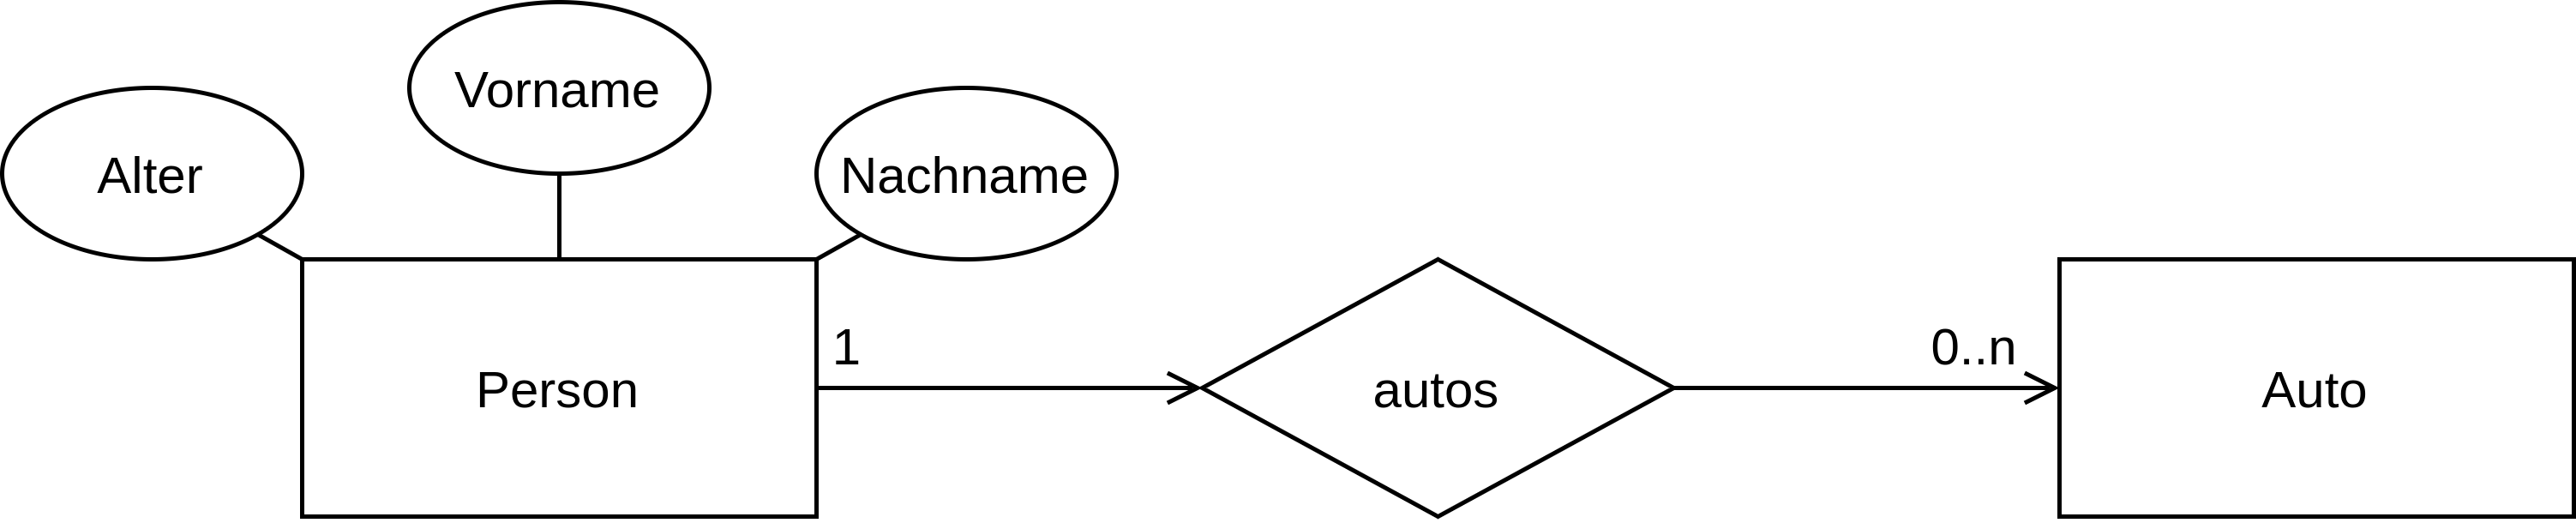
\includegraphics[width=\textwidth]{images/ERM-Entity}
	\captionof{figure}[Beispiel für eine Entity im \acrshort{erm}]{Beispiel für eine Entity mit Attributen und einer Beziehung}
	\label{fig:erm-entity}
\end{center}
\subsection*{Attribute}
Attribute können dabei eindeutig, optional oder mehrwertig sein. Die Unterscheidung zwischen Datum, Zahl oder Zeichenkette wird in einem \acrlong{erm} nicht dargestellt.
\begin{center}
	\captionsetup{type=figure}
	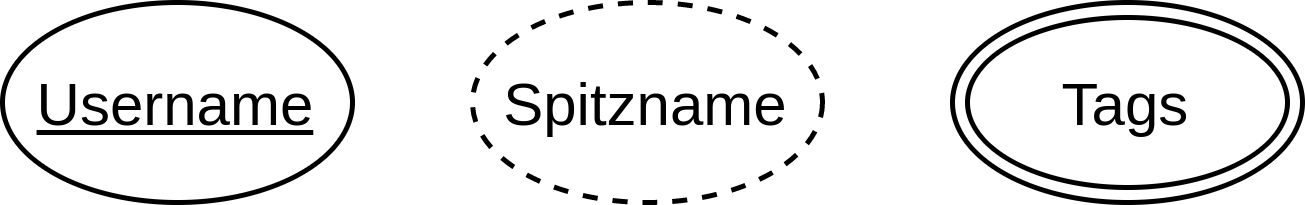
\includegraphics[width=10cm]{images/ERM-Attributes}
	\captionof{figure}[Verschiedene Arten von Attributen im \acrshort{erm}]{Attribute (v.l.): eindeutig, optional und mehrwertig}
	\label{fig:erm-attributes}
\end{center}
% Hauptteil
\section{Entwurf}
Hauptfrage:
Wie kann man das beste Framework für die Oberfläche auswählen?
Wie wählt man die beste API aus? (Kiwi, Google etc) -> Vergleichstabelle aus Anforderungen
\subsection{Datenmodell}
Das \acrlong{erm} für das Datenmodell wurde hier aufgeteilt in Suchanfrage (SearchRequest) und Antwort der Anwendung (SearchResult).
\begin{center}
	\captionsetup{type=figure}
	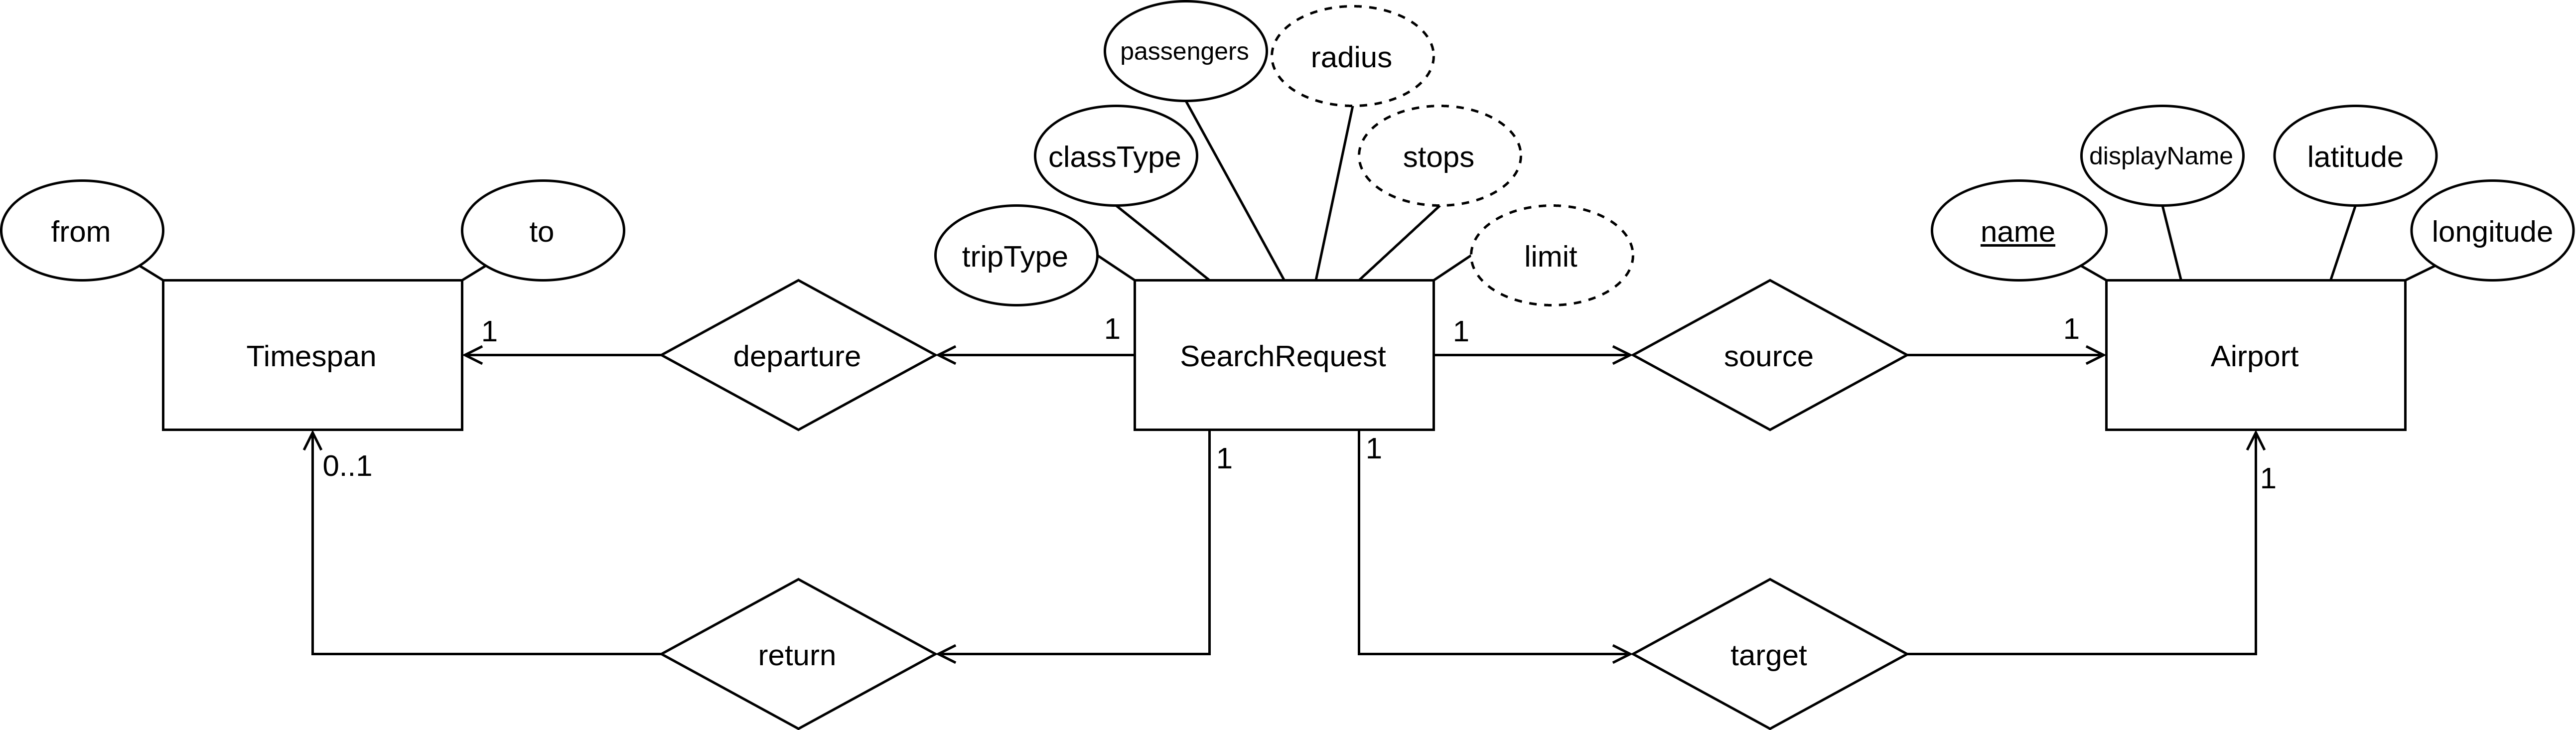
\includegraphics[width=\textwidth]{images/datamodel-SearchRequest}
	\captionof{figure}[\acrshort{erm} SearchRequest]{\acrlong{erm} des SearchRequest Objekts}
\end{center}
\begin{center}
	\captionsetup{type=figure}
	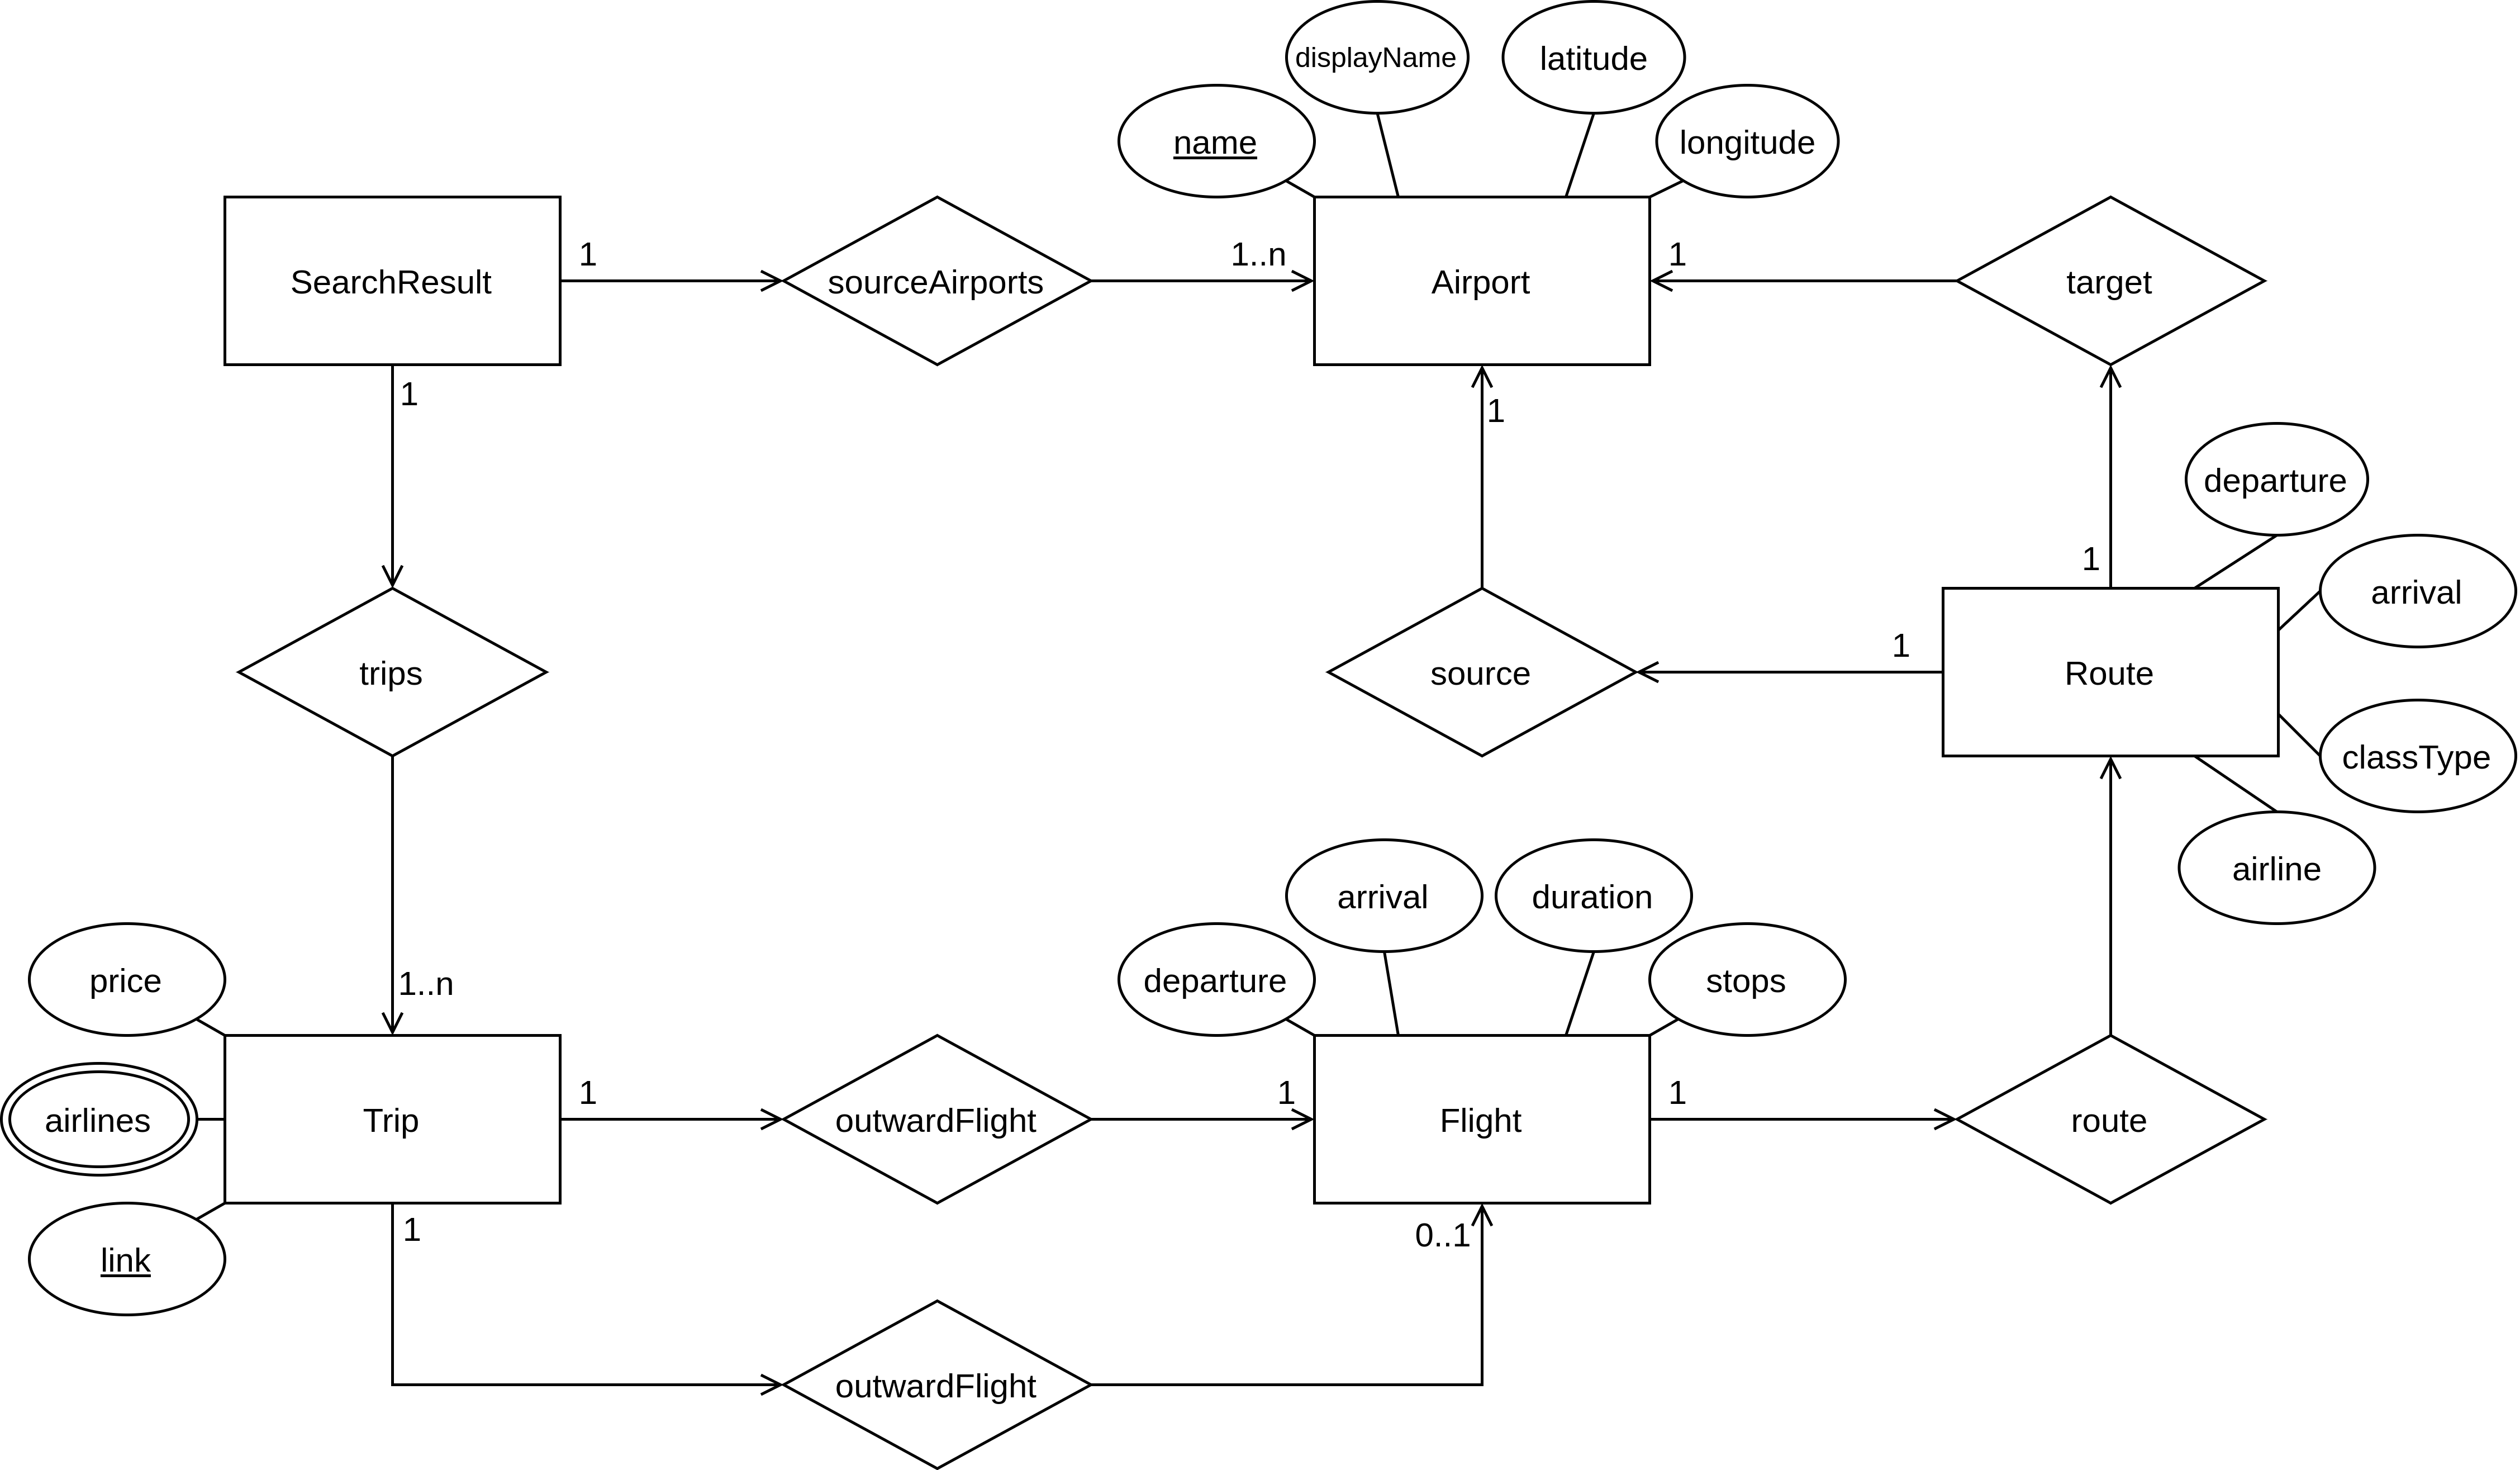
\includegraphics[width=\textwidth]{images/datamodel-SearchResult}
	\captionof{figure}[\acrshort{erm} SearchResult]{\acrlong{erm} des SearchResult Objekts}
\end{center}
% Umsetzung
\section{Implementierung}
Wie portabel ist das System? -> Docker, React -> static html+js
\section{Testing}
Unit tests?
How to test external api?
Aspects of an API: speed? maybe Beständigkeit in der Speed?
% Ende
\section{Zusammenfassung}
\subsection{Ausblick}
-> Monitor speed of my requests!!
% Literaturverzeichnis
\newpage
% set interlinepenalty to not split entries on page break
\bibliographystyle{apacite}
\bibliography{paper}
\end{document}